\documentclass{article}
\usepackage[letterpaper]{geometry}
\geometry{verbose,tmargin=1in,bmargin=1in,lmargin=1in,rmargin=1in}

\usepackage[utf8]{inputenc}
\usepackage{amsmath}
\usepackage{amssymb}
\usepackage{listings}
\usepackage{graphicx}
\usepackage{enumitem}
\usepackage{caption}
\usepackage{subcaption}
\usepackage{array}
\usepackage{tabularx}

\newcolumntype{P}[1]{>{\centering\arraybackslash}p{#1}}

\title{CIS 419/519: Homework 3}
\author{Jiatong Sun}
\date{}

\begin{document}
    \maketitle
	Although the solutions are entirely my own, I consulted with the following people and sources while working on this homework: $Junfan Pan$, $Zhuoyu He$, $Yuchen Sun$, $Yupeng Li$, $Jing Zhao$, $Tianjia Zhu$\\ 
	$https://scikit-learn.org/stable/modules/generated/sklearn.model_selection.KFold.html$
    
    \section{Logistic Regression}
    	\begin{enumerate}
    	\item [1.3]Analysis
    	
    	\begin{figure}[h!]
     	\centering
     	\begin{subfigure}[b]{0.44\textwidth}
         	\centering
         	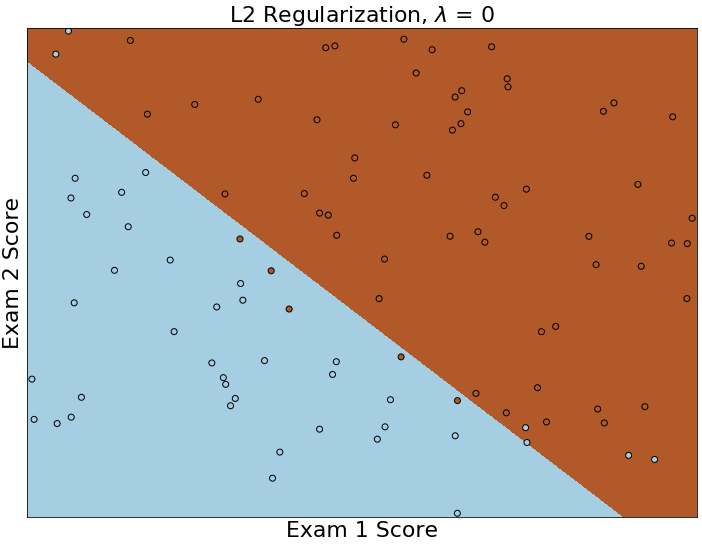
\includegraphics[width=\textwidth]
         	{Problem_1_3/fig_L2_1.png}
         	\caption{$\lambda = 0, regNorm = 2$}
         	\label{fig:L2_1}
     	\end{subfigure}
     	\hfill
     	\begin{subfigure}[b]{0.44\textwidth}
         	\centering
         	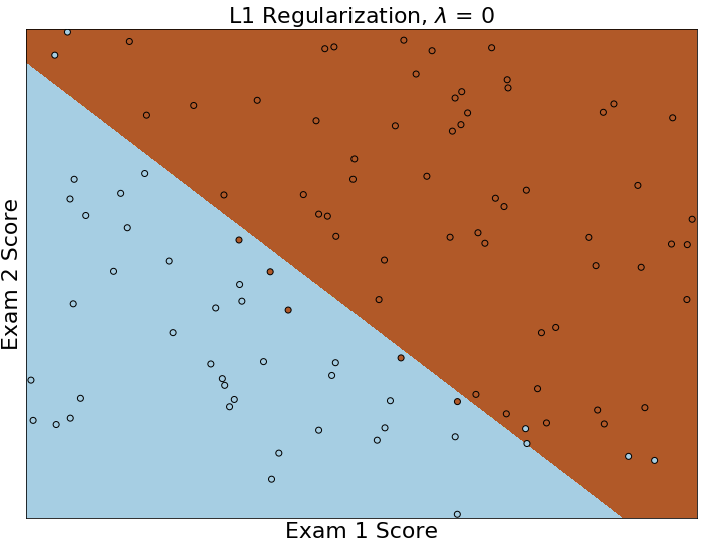
\includegraphics[width=\textwidth]
         	{Problem_1_3/fig_L1_1.png}
         	\caption{$\lambda = 0, regNorm = 1$}
         	\label{fig:L1_1}
     	\end{subfigure}
     	\caption{$\lambda=0$}
		\end{figure}
		
    	\begin{figure}[h!]
     	\centering
     	\begin{subfigure}[b]{0.44\textwidth}
         	\centering
         	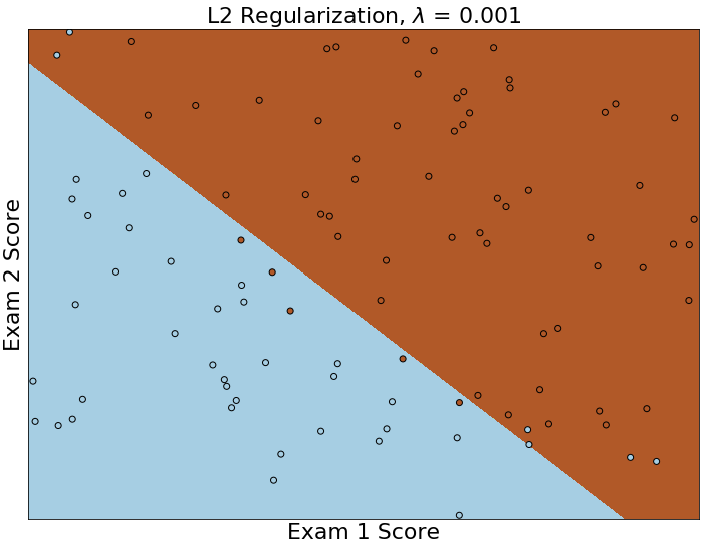
\includegraphics[width=\textwidth]
         	{Problem_1_3/fig_L2_2.png}
         	\caption{$\lambda = 0.001, regNorm = 2$}
         	\label{fig:L2_2}
     	\end{subfigure}
     	\hfill
     	\begin{subfigure}[b]{0.44\textwidth}
         	\centering
         	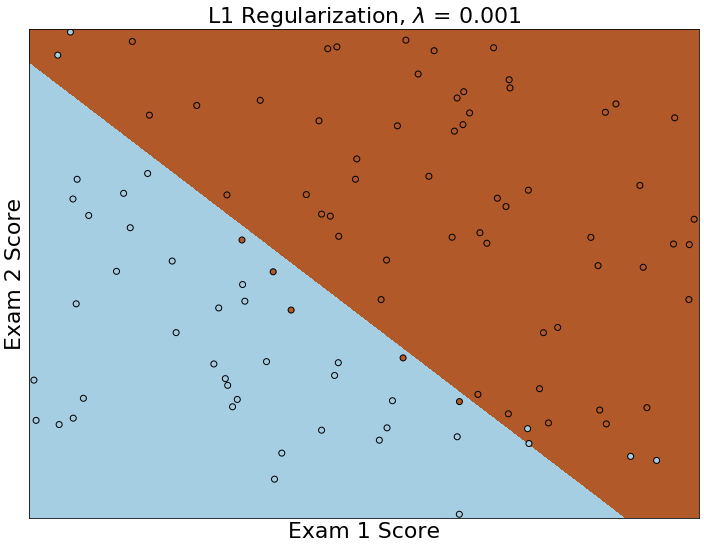
\includegraphics[width=\textwidth]
         	{Problem_1_3/fig_L1_2.png}
         	\caption{$\lambda = 0.001, regNorm = 1$}
         	\label{fig:L1_2}
     	\end{subfigure}
     	\caption{$\lambda=0.001$}
		\end{figure}
		
    	\begin{figure}[h!]
     	\centering
     	\begin{subfigure}[b]{0.44\textwidth}
         	\centering
         	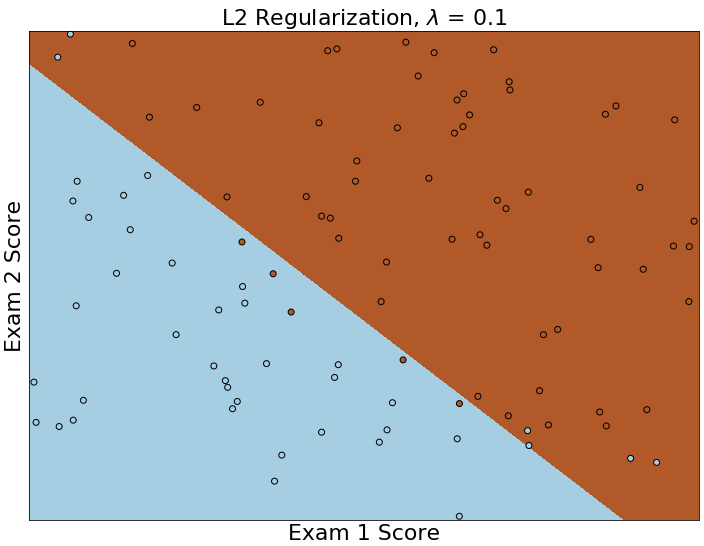
\includegraphics[width=\textwidth]
         	{Problem_1_3/fig_L2_3.png}
         	\caption{$\lambda = 0.1, regNorm = 2$}
         	\label{fig:L2_3}
     	\end{subfigure}
     	\hfill
     	\begin{subfigure}[b]{0.44\textwidth}
         	\centering
         	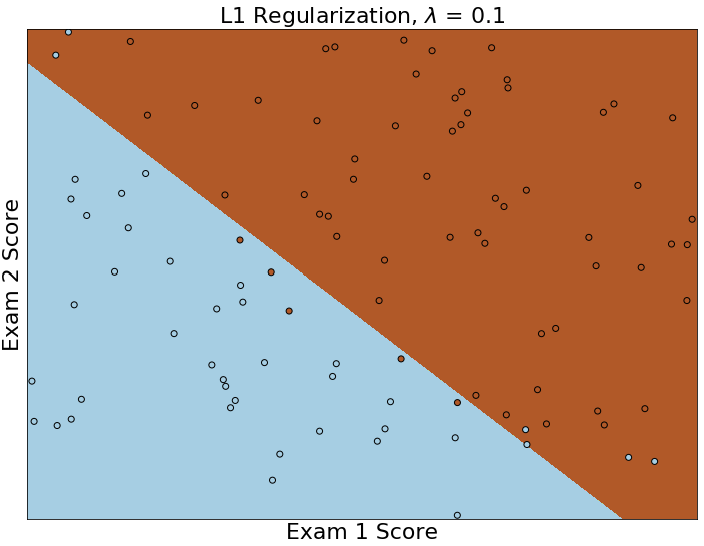
\includegraphics[width=\textwidth]
         	{Problem_1_3/fig_L1_3.png}
         	\caption{$\lambda = 0.1, regNorm = 1$}
         	\label{fig:L1_3}
     	\end{subfigure}
     	\caption{$\lambda=0.1$}
		\end{figure}
		
    	\begin{figure}[h!]
     	\centering
     	\begin{subfigure}[b]{0.44\textwidth}
         	\centering
         	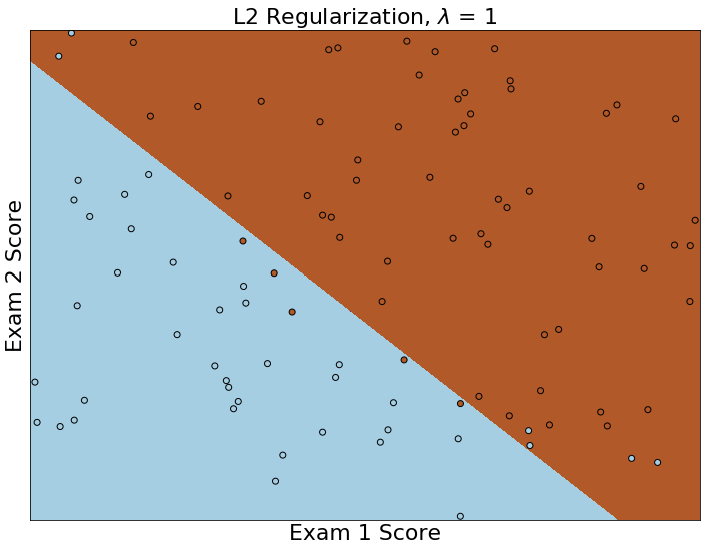
\includegraphics[width=\textwidth]
         	{Problem_1_3/fig_L2_4.png}
         	\caption{$\lambda = 1, regNorm = 2$}
         	\label{fig:L2_4}
     	\end{subfigure}
     	\hfill
     	\begin{subfigure}[b]{0.44\textwidth}
         	\centering
         	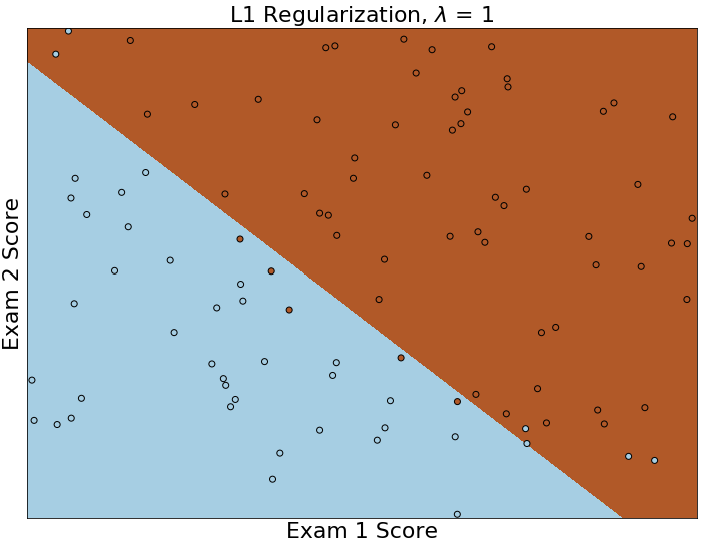
\includegraphics[width=\textwidth]
         	{Problem_1_3/fig_L1_4.png}
         	\caption{$\lambda = 1, regNorm = 1$}
         	\label{fig:L1_4}
     	\end{subfigure}
     	\caption{$\lambda=1$}
		\end{figure}
		
    	\begin{figure}[h!]
     	\centering
     	\begin{subfigure}[b]{0.44\textwidth}
         	\centering
         	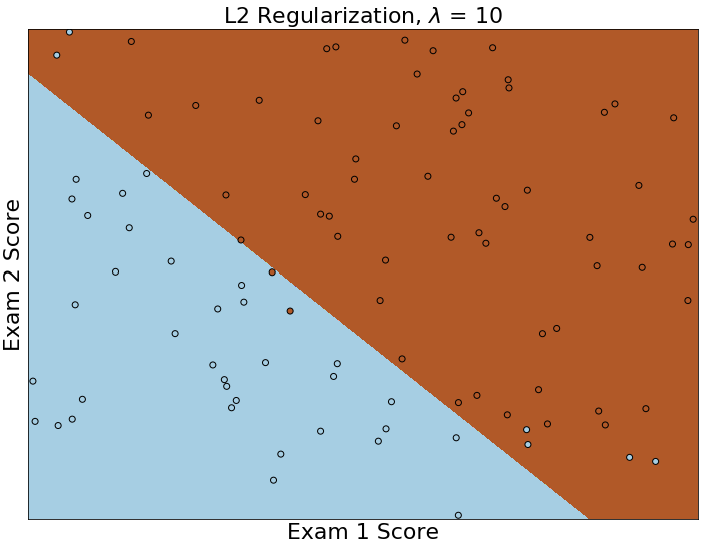
\includegraphics[width=\textwidth]
         	{Problem_1_3/fig_L2_5.png}
         	\caption{$\lambda = 10, regNorm = 2$}
         	\label{fig:L2_5}
     	\end{subfigure}
     	\hfill
     	\begin{subfigure}[b]{0.44\textwidth}
         	\centering
         	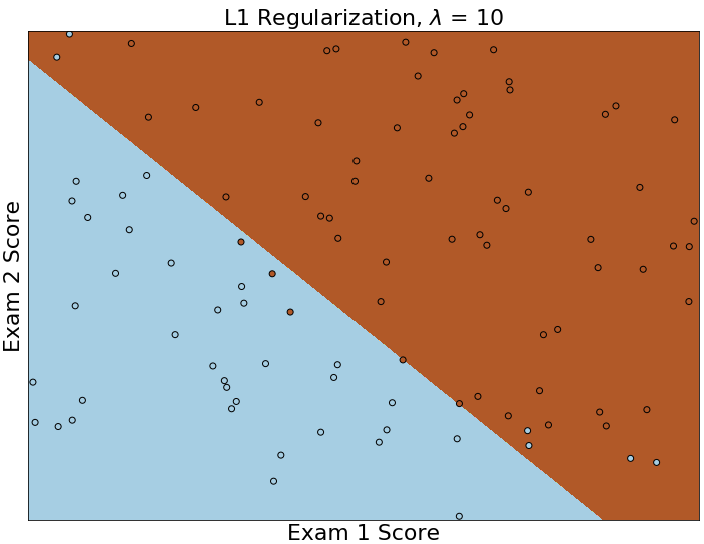
\includegraphics[width=\textwidth]
         	{Problem_1_3/fig_L1_5.png}
         	\caption{$\lambda = 10, regNorm = 1$}
         	\label{fig:L1_5}
     	\end{subfigure}
     	\caption{$\lambda=10$}
		\end{figure}
		
    	\end{enumerate}

	\newpage
	\noindent
	\textbf{Conclusion: }\\
	As the $\lambda$ increases, the border slightly moves to bottom left corner, which means more data are recognized as 1. This is because a bigger $\lambda$ causes the regularization term to be bigger and the convergence to be more quick, and thus the boarder stops moving at a relatively small iteration number. For l1 and L2, when $\lambda$ is small, the difference is hard to observe; but when $\lambda$ is greater than 1, L2 norm converges more quickly than L1 norm and thus its boarder is more close to the bottom left corner.
	
	
	
	
    \section{Comparing Algorithms} 
    	\begin{enumerate}
    	\item [2.2]Comparing Algorithms\\
    	\begin{center}
    	\begin{tabular}
    	{ |P{1.7cm}||P{1.8cm}|P{1.8cm}|P{1.5cm}| P{5cm}| }
		\hline
		\multicolumn{5}{|c|}
		{\textbf{Data Set Description}} \\
 		\hline
		 	\textbf{Data Set} & 
		 	\textbf{number of features} & 
		 	\textbf{number of instances} & 
		 	\textbf{missing data} & 
		 	\textbf{feature properties}\\
 		\hline
 			wdbc & 30 & 569 & No &
 			Computed from a digitized image of a fine 	
 			needle aspirate (FNA) of a breast mass\\
 		\hline
 			retinopathy & 19  & 1151 & No &
 			Represent either a detected lesion, a 
 			descriptive feature of a anatomical part
 			or an image-level descriptor\\
 		\hline
 			diabetes & 8 & 768 & No & 
 			Predict whether or not a patient has diabetes 
 			based on certain diagnostic measurements\\
 		\hline
		\end{tabular}
    	\end{center}

		Setup: \\
		All of the following learning processes use those parameters: \\
		$\alpha=0.001$, $maxNumIters=10000$,  $\epsilon=0.0001$, 3 trials, 5 folders\\		
		
		Result:\\
		\begin{center}
		\begin{tabularx}{0.8\textwidth} { 
 			| >{\centering\arraybackslash}X 
  			| >{\centering\arraybackslash}X 
   			| >{\centering\arraybackslash}X | }
   			\hline
   			\multicolumn{3}{|c|}
   			{\textbf{wdbc data set}}\\
 			\hline
 					 & $\lambda=1$ & $\lambda=10$ \\
 			\hline
 			Logistic Regression L1 & 0.9701 & 0.9701\\
 			\hline
 			Logistic Regression L2 & 0.9748 & 0.9736\\
 			\hline
 			Adagrad L1 & 0.6274 & 0.6290\\
 			\hline
 			Adagrad L2 & 0.9467  & 0.8594\\
			\hline
		\end{tabularx}  
		\end{center} 
		
		\begin{center}
		\begin{tabularx}{0.8\textwidth} { 
 			| >{\centering\arraybackslash}X 
  			| >{\centering\arraybackslash}X 
   			| >{\centering\arraybackslash}X | }
   			\hline
   			\multicolumn{3}{|c|}
   			{\textbf{retinopathy data set}}\\
 			\hline
 					 & $\lambda=1$ & $\lambda=10$ \\
 			\hline
 			Logistic Regression L1 & 0.7324 & 0.6904\\
 			\hline
 			Logistic Regression L2 & 0.7261 & 0.6901\\
 			\hline
 			Adagrad L1 & 0.5308 & 0.5308\\
 			\hline
 			Adagrad L2 & 0.5995 & 0.5946\\
			\hline
		\end{tabularx}  
		\end{center}
		
		\begin{center}
		\begin{tabularx}{0.8\textwidth} { 
 			| >{\centering\arraybackslash}X 
  			| >{\centering\arraybackslash}X 
   			| >{\centering\arraybackslash}X | }
   			\hline
   			\multicolumn{3}{|c|}
   			{\textbf{diabetes data set}}\\
 			\hline
 					 & $\lambda=1$ & $\lambda=10$ \\
 			\hline
 			Logistic Regression L1 & 0.7704 & 0.7687\\
 			\hline
 			Logistic Regression L2 & 0.7717 & 0.7682\\
 			\hline
 			Adagrad L1 & 0.6510 & 0.6510\\
 			\hline
 			Adagrad L2 & 0.7214 & 0.6510\\
			\hline
		\end{tabularx}  
		\end{center} 
		
		\newpage
    	\item [2.3]
    	Understanding Regularization and Adagrads\\
    	
    	Setup:
    	All of the following learning curves are generated on "wdbc.csv"
    	
    	\begin{figure}[h!]
     	\centering
     	\begin{subfigure}[b]{0.3\textwidth}
         	\centering
         	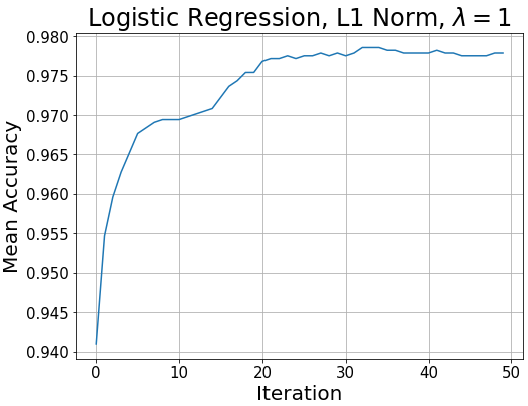
\includegraphics[width=\textwidth]
         	{Problem_2_3/logistic_L1_1.png}
         	\caption{L1, $\lambda=1,\alpha=0.001$}
         	\label{fig:LR_L1_1}
     	\end{subfigure}
     	\hfill
     	\begin{subfigure}[b]{0.3\textwidth}
         	\centering
         	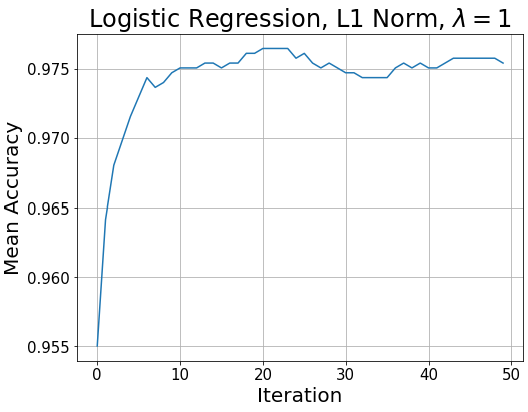
\includegraphics[width=\textwidth]
         	{Problem_2_3/logistic_L1_2.png}
         	\caption{L1, $\lambda=1,\alpha=0.01$}
         	\label{fig:LR_L1_2}
     	\end{subfigure}
     	\hfill
     	\begin{subfigure}[b]{0.3\textwidth}
         	\centering
         	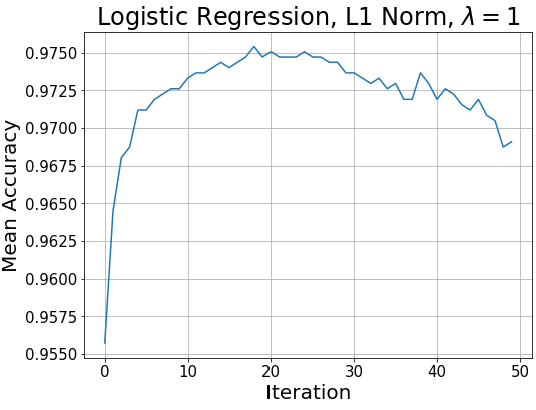
\includegraphics[width=\textwidth]
         	{Problem_2_3/logistic_L1_3.png}
         	\caption{L1, $\lambda=1,\alpha=0.1$}
         	\label{fig:LR_L1_3}
     	\end{subfigure}
		\hfill
     	\begin{subfigure}[b]{0.3\textwidth}
         	\centering
         	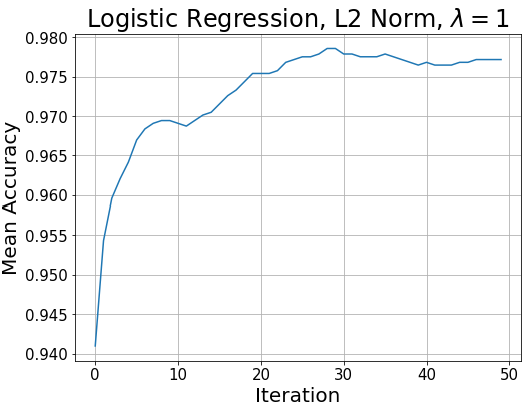
\includegraphics[width=\textwidth]
         	{Problem_2_3/logistic_L2_1.png}
         	\caption{L2, $\lambda=1,\alpha=0.001$}
         	\label{fig:LR_L2_1}
     	\end{subfigure}
     	\hfill
     	\begin{subfigure}[b]{0.3\textwidth}
         	\centering
         	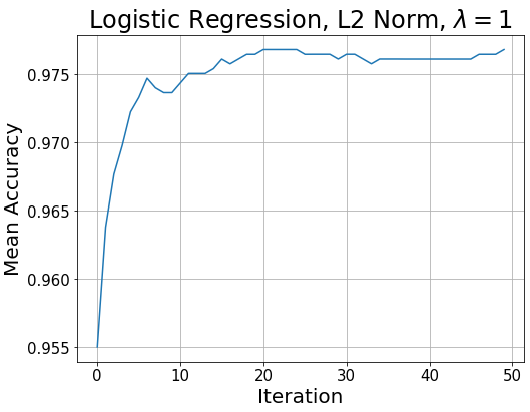
\includegraphics[width=\textwidth]
         	{Problem_2_3/logistic_L2_2.png}
         	\caption{L2, $\lambda=1,\alpha=0.01$}
         	\label{fig:LR_L2_2}
     	\end{subfigure}
     	\hfill
     	\begin{subfigure}[b]{0.3\textwidth}
         	\centering
         	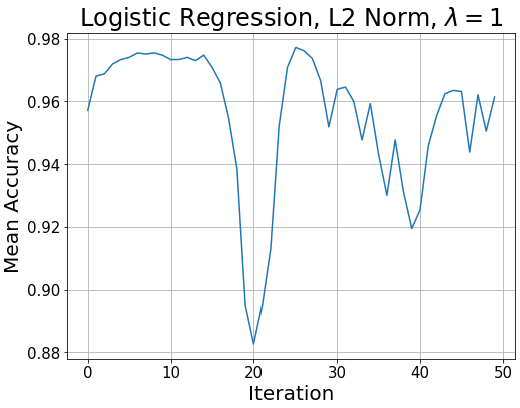
\includegraphics[width=\textwidth]
         	{Problem_2_3/logistic_L2_3.png}
         	\caption{L2, $\lambda=1,\alpha=0.1$}
         	\label{fig:LR_L2_3}
     	\end{subfigure}
     	\hfill
     	\begin{subfigure}[b]{0.3\textwidth}
         	\centering
         	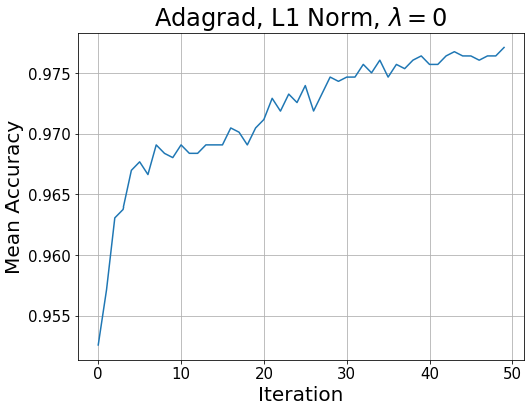
\includegraphics[width=\textwidth]
         	{Problem_2_3/Adagrad_L1_1.png}
         	\caption{L1, $\lambda=0,\alpha=0.01$}
         	\label{fig:ADA_L1_1}
     	\end{subfigure}
     	\hfill
     	\begin{subfigure}[b]{0.3\textwidth}
         	\centering
         	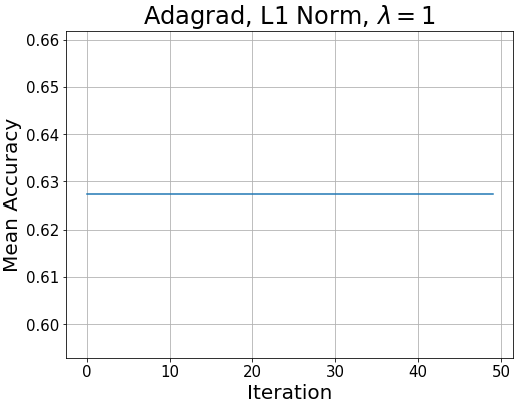
\includegraphics[width=\textwidth]
         	{Problem_2_3/Adagrad_L1_2.png}
         	\caption{L1, $\lambda=1,\alpha=0.01$}
         	\label{fig:ADA_L1_2}
     	\end{subfigure}
     	\hfill
     	\begin{subfigure}[b]{0.3\textwidth}
         	\centering
         	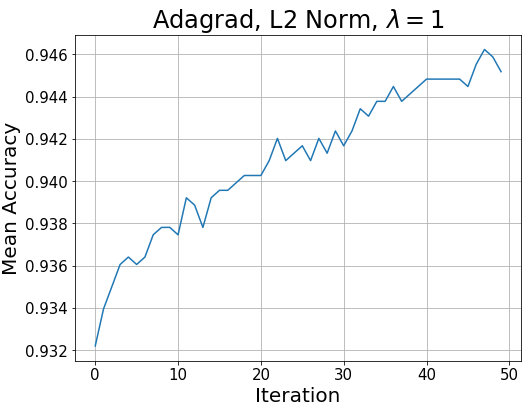
\includegraphics[width=\textwidth]
         	{Problem_2_3/Adagrad_L2_1.png}
         	\caption{L2, $\lambda=1,\alpha=0.001$}
         	\label{fig:ADA_L2_1}
     	\end{subfigure}
     	\caption{Learning Curves}
		\end{figure}
		\noindent
		\textbf{Conclusion:}
		\begin{itemize}
     		\item From the first two rows of graphs, we can  discover the influence of the learning rate $\alpha$. When the learning rate goes bigger, learning process becomes faster, but a too big $\alpha$ may result in an overshooting, and thus make the mean accuracy to drop down at some point.
     		\item From \ref{fig:ADA_L1_1} and \ref{fig:ADA_L1_2}, we can discover the influence of regularization. When $\lambda=0$, the learning accuracy can go high continuously. But for $\lambda=1$, the learning performance will remain a low level. This is because the regularization parameter is set too big and prevent over-fitting excessively so the learning can not happen.
     		\item From the first two rows of graphs, we can discover the difference between L1 norm and L2 norm. When the learning rate $\alpha$ goes bigger, L2 norm is more sensitive than L1 norm, which is because the regularization term takes more ratio in L2 norm than in L1 norm.
     		\item From the first two rows and the last row, we can discover the difference between a fixed learning rate and adagrad. When using a fixed learning rate, the learning curve is much more smooth, while using adagrad makes the curve have many spikes. This is because adagrad adjusts gradient according to the frequency of feature properties and only goes a large step when the current feature has a high frequency. So there is more oscillation in the learning process in adagrad than with a fixed learning rate.
  		\end{itemize}		
    	\end{enumerate}
       
        
\end{document}